\subsection{JIT Emulator}
\label{section:jit-arch}

The JIT emulator functions by partitioning the program, as it is executed, into source blocks. These blocks are compiled into corresponding x86 host blocks and stored in the translation cache. Each host block terminates by returning an address, corresponding to the exiting MIPS program counter (PC). For blocks without a terminating jump, this will be the subsequent instruction. The system will then execute the block at the desired PC, compiling a new host block if required. This architecture is outlined in \autoref{figure:jit-arch}.

\begin{figure}[H]
    \centering
    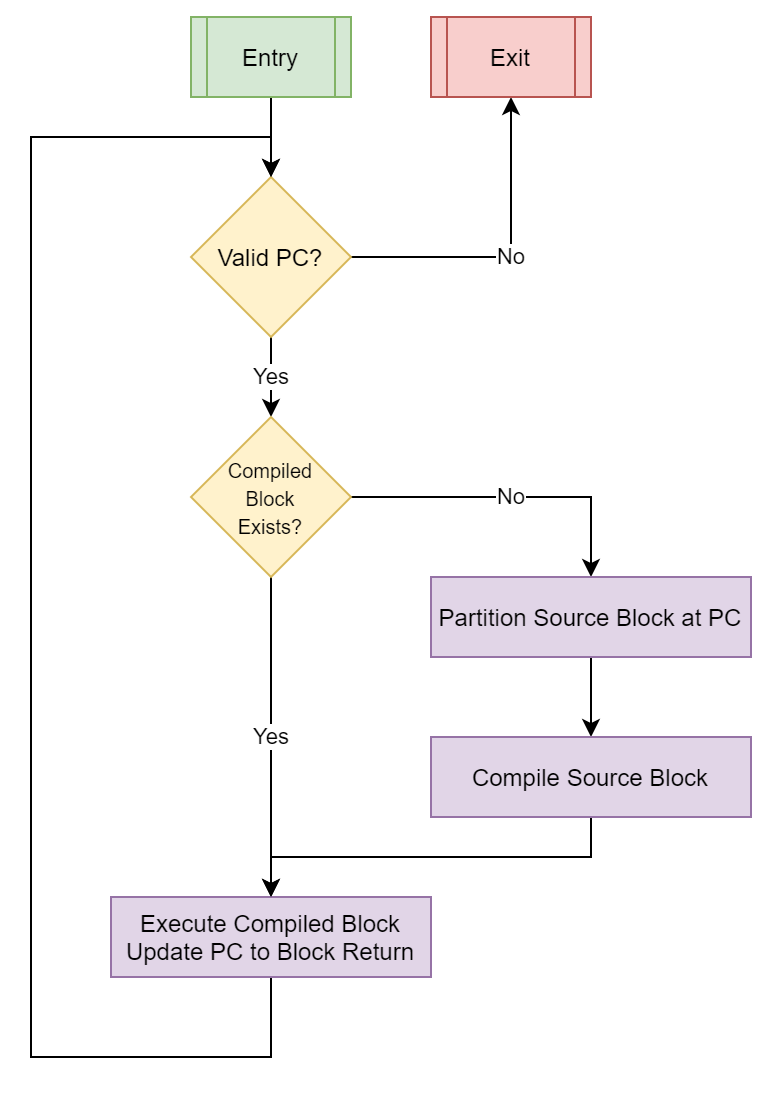
\includegraphics[width=0.5\linewidth]{diagrams/jit.png}
    \caption{Top level architecture of the JIT emulator.}
    \label{figure:jit-arch}
\end{figure}

This architecture was chosen as compiled host blocks cannot have a jump compiled directly to the desired PC, as the destination may not be compiled yet.

The JIT emulator is composed of the following components:

\begin{itemize}
    \item \textbf{Runtime}

    The runtime is the top level JIT emulation system and ties together all the other JIT components. When provided with a MIPS program the runtime will then emulate it by partitioning it into blocks and compiling them with the compiler. These compiled host blocks are stored in a cache and re-used on subsequent executions.

    \item \textbf{Compiler}

    The compiler is used to convert source MIPS-1 blocks into host x86 blocks.

    \item \textbf{Assembler}

    The assembler is responsible for encoding the desired \texttt{x86} instructions into an internal buffer, which can then be copied into the executable memory buffer once compilation of a block is complete. It makes heavy usage of templates and \texttt{constexpr} evaluation to offload as much work as possible to \texttt{C++} compile time, increasing the runtime performance. It is currently designed to support 8-bit, 16-bit and 32-bit \texttt{x86} instructions.

    \item \textbf{Block Partitioner}

    The block partitioner is responsible for partitioning the program into a source block for a given address. Source blocks are terminated when a jump instruction is encountered, however the following instruction is also included in order to support the MIPS delay slot. Other partitioning schemes are possible such as a single instruction, however shorter blocks lead to more compilation overhead.

    \item \textbf{Register File}

    The register file described in \autoref{section:interpreter-reg-file} provides the runtime and compiler with a means of emulating the MIPS register file. The current implementation uses an in memory model, where a C++ array represents the MIPS register bank. Translated x86 instructions load and store this array when they need to emulate a MIPS register modification. The special \texttt{hi} and \texttt{lo} registers in MIPS are mapped internal to \texttt{\$32} and \texttt{\$33} respectively, so the same compilation architecture can be used. This memory model provides for fast compile times but subpar execution times, as the contents must be written back after every instruction, causing in some cases large overhead.

    Other solutions can be explored such as direct register mapping or a hybrid model \cite{mark-probst-dbt}; these should yield increase execution performance, but potentially at the cost of worse compiler performance. These will also increase the complexity of the solution.

    The compiler omits any instructions that would cause a write to \texttt{\$0}, preserving its constant zero value.

    \item \textbf{Memory Map}

    Instead of attempting to generate native x86 code to model the MIPS memory space, the JIT emulator re-uses the same \texttt{MemoryMap} component created for the interpreter runtime described in \autoref{section:interpreter-mem-map} to emulate the memory space. The x86 code is then compiled with calls to the existing C++ implementations.
\end{itemize}
